%%%%%%%%%%%%%%%%%%%%%%%%%%%%%%%%%%%%%%%%%

% Simple Sectioned Essay Template
% LaTeX Template
%
% This template has been downloaded from:
% http://www.latextemplates.com
%
% Note:
% The \lipsum[#] commands throughout this template generate dummy text
% to fill the template out. These commands should all be removed when 
% writing essay content.
%
%%%%%%%%%%%%%%%%%%%%%%%%%%%%%%%%%%%%%%%%%

%----------------------------------------------------------------------------------------
%	PACKAGES AND OTHER DOCUMENT CONFIGURATIONS
%----------------------------------------------------------------------------------------

\documentclass[12pt]{article} % Default font size is 12pt, it can be changed here

\usepackage{geometry} % Required to change the page size to A4
\usepackage{subfigure}
\usepackage{placeins}
\usepackage{placeins}
\usepackage{hyperref}
\geometry{a4paper} % Set the page size to be A4 as opposed to the default US Letter

\usepackage{graphicx} % Required for including pictures

\usepackage{float} % Allows putting an [H] in \begin{figure} to specify the exact location of the figure
\usepackage{amssymb} % Allows putting an [H] in \begin{figure} to specify the exact location of the figure
\usepackage{wrapfig} % Allows in-line images such as the example fish picture

\usepackage{lipsum} % Used for inserting dummy 'Lorem ipsum' text into the template

\linespread{1.2} % Line spacing

%\setlength\parindent{0pt} % Uncomment to remove all indentation from paragraphs

\graphicspath{{./Pictures/}} % Specifies the directory where pictures are stored

\begin{document}
\title{Byzantine agreement task}
\author{Inge Becht}
\date{\today}

\maketitle
 \begin{itemize}
     \item IP-address of ss64.com : 216.92.29.160\\
           IP-address of the sending computer : 145.18.214.201\\
    \item 8 HTTP GET messages were sent.
        I used filter \emph{http and ip.src == 145.18.214.201 and ip.dts ==
        216.92.29.160}\
    \item 
        I chose the emph{GET /bash.ping.html HTTP/1.1} message. The included
        protocols were:\\
        \begin{itemize}
            \item Internet Protocol version 4 (IPv4)
            \item Transmission Control Protocol
            \item Hypertext Transfer Protocol (HTTP)
        \end{itemize}
    \item If by your computer is meant the computer from which te dump is taken: 
        8 HTTP OK messages from ss64.com(filter : \emph{http and ip.src ==
        145.18.214.201 and ip.dst == 216.92.29.160} )
    \item{ By filtering on \emph{http} the first two messages are a HHTP GET and
            HTTP OK messags. Then, choosing the \emph{Seconds since Previously
            Displayed Packet option} in the time display you get approximately
            0.4345 seconds.
         }
    \item Yes, 6 images were sent:
        \begin{itemize}
            \item ss64.gif
            \item bash-l.gif
            \item syntax-r.gif
            \item top-4.gif
            \item roll-left.png
            \item roll-right.png
        \end{itemize}
    TODO\item 
    \item 
        Computer sent 38 packets(total of 5650 bytes) to the server and
        ss64.com sent
        39 packets(total of 32908 bytes) to the computer
        There is a lot more received by the computer than sent, this because all the images needed to
        be sent to the computer and the computer only asked for permission to
        get this content.
   \item
    \begin{figure}[h!]
        \centering
        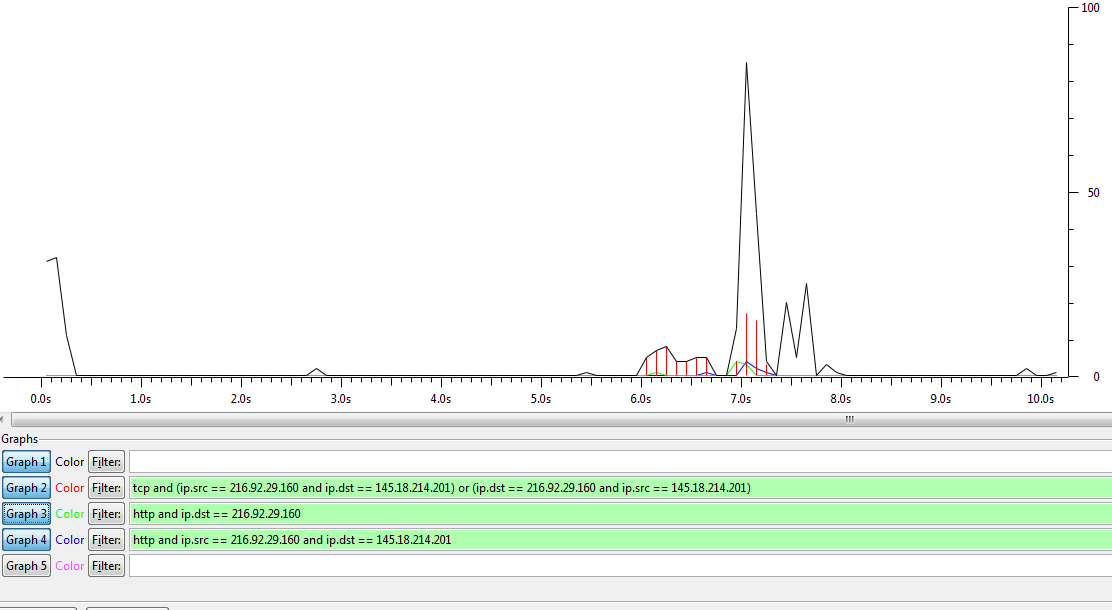
\includegraphics[width=0.3\textwidth]{data.png}
        \caption{Packet distribution}
        \label{ref:simple}
    \end{figure}

    See figure \ref{ref:simple} for the graph. This graph seems not all that
    clear to me so also see fiugre \ref{ref:simple2} for the HTTP messages sent between
    ss64.com and the computer. Here the seems to be consistent with
    earlier answers( 8 HTTP GET messages were sent and 8 received)


\begin{figure}[h!]
    \centering
    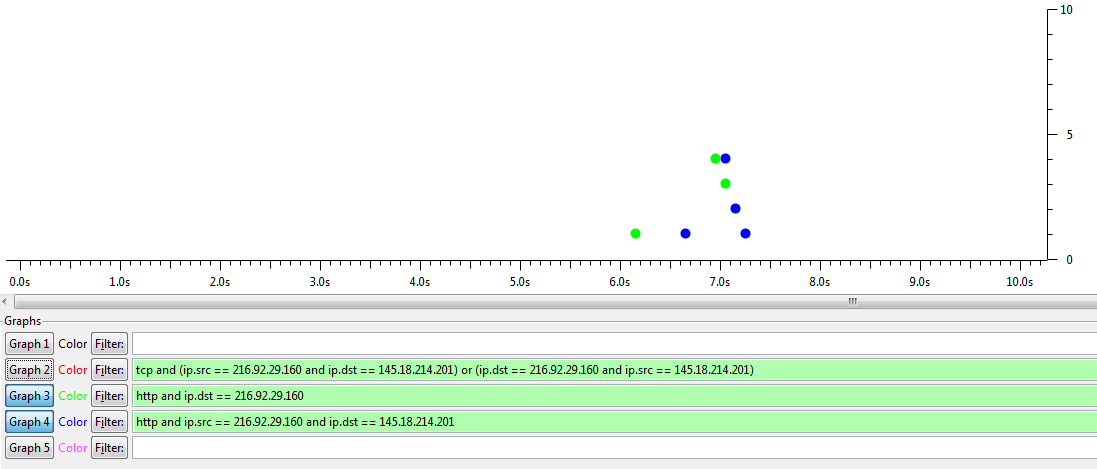
\includegraphics[width=0.3\textwidth]{data2.png}
    \caption{HTTP GET and OK distribution between computer and ss64.com}
    \label{ref:simple2}
\end{figure}

    \item The passwords sent are \emph{wrong!} and \emph{network}
        First I filtered on \emph{http} to show all readible data. Here I found
        the ip 145.100.102.253 making a HTTP GET request towards ip
        145.00.102.153. So the first ip belonged to the computer and the other
        ip to some site that the computer tried to connect to. In the HTML sent to the
        compputer I could read when the user did not have acces to the page
        tried to visit and when he did (entry 13 and 25 respectively). So then I
        read the requests and found the authorization section with the
        credentials and the bits that was different and gave the ability to
        receive the requested page.
        The correct password is network. This because after applying this
        password the computer receives the site contect that shows it was the
        right password. I myself went to
        \url{http://gaia.cs.umass.edu/wireshark-labs/protected_pages/HTTP-wireshark-file5.html} as well to check if this
        password worked (together with the username wireshark-student) and it
        worked.

 \end{itemize}


\end{enumerate}
\end{document}

